\documentclass[a4paper,11pt]{article}
\usepackage[utf8]{inputenc}
\usepackage[ngerman]{babel}
\usepackage{geometry}
\geometry{left=25mm, top=20mm, right=25mm, headheight=14pt}
\usepackage[onehalfspacing]{setspace}
\usepackage{graphicx}
\usepackage{indentfirst}
\usepackage{lastpage}
\usepackage{pdfpages}
\usepackage{listings}
\usepackage{textcomp}
\usepackage{xcolor}
\usepackage{hyperref}

\newcommand*{\mybox}[2]{\colorbox{#1!30}{\parbox{.98\linewidth}{#2}}}
\hypersetup{
	colorlinks,
	citecolor=black,
	filecolor=black,
	linkcolor=black,
	urlcolor=black
}


\definecolor{background}{gray}{0.5}
\newcommand{\code}[1]{\colorbox{background}{\texttt{#1}}}

\lstset{ basicstyle=\small\ttfamily }
\lstset{
	backgroundcolor = \color{background}
,
	numbers=left,
	breaklines=true
}
\lstset{literate=%
	{Ö}{{\"O}}1
	{Ä}{{\"A}}1
	{Ü}{{\"U}}1
	{ß}{{\ss}}1
	{ü}{{\"u}}1
	{ä}{{\"a}}1
	{ö}{{\"o}}1
}


\pagenumbering{arabic}


\newcommand{\sign}[1]{%
	\begin{tabular}[t]{@{}l@{}}
		\makebox[2in]{\dotfill}\\
		\strut#1\strut
	\end{tabular}%
}

\begin{document}
\begin{titlepage}
	\hfill
	\vfill
	{
	\begin{center}
	\huge{\textbf{Entwicklung eines Softwaresystems 2019}}
	---------\\
	\large{\textbf{Landkartenerstellung}}
	\end{center}
	}

	\vfill
{\textit{\\Vorgelegt von:\\}}
	{Christoph Schirmel\\}
	{Pr\"ufungsnummer: }
	{101-20510\\}
	{Ausbildungsbetrieb: }
	{CAE Elektronik GmbH}
\end{titlepage}
\tableofcontents
\newpage

\includepdf{ErklaerungUnterschrieben.pdf}
{\parindent0pt
\section{Aufgabenbeschreibung}
Die MATSEgraphic AG stellt den Auftrag zur Erstellung von schemenhaften Karten auf Basis vorgegebener Kennwerte. Ausgangspunkt ist eine gegebene Menge an beliebigen Staaten mit
ihrer realen Lage, angegeben in L\"aengen- und Breitengrad, ihren realen Nachbarschaftsbeziehungen und dem jeweiligen Kennwert. Die Staaten sollen auf der erstellten Karte als Kreis
dargestellt werden. Die Gr\"oesse des Kreises ist proportional zu der gegebenen Kenngr\"oesse, also wird der Kreis f\"ur gr\"oessere Kennwerte gr\"oesser und f\"ur kleinere Kennwerte kleiner.
In der erstellten Karte sollen die Lage- und Nachbarschaftsbeziehungen so gut wie m\"oglich erhalten bleiben. Die Qualit\"at der Karte bemisst sich insgesamt am Abstand der L\"ander zueinander, sowie den Lage-
und Nachbarschaftsbeziehungen. \"Uberschneidungen und zu grosse Abst\"ande mindern die Qualit\"at der Karte und sollen vermieden werden. Die numerische Gr\"ossenordnung der Karte kann beliebig skaliert werden und hat keinen 
unmittelbaren Einfluss auf die Qualit\"at der Karte, welche lediglich durch die oben beschriebenen Kriterien bestimmt wird.

\vspace{10mm}
\textbf{Beispiel:}

\begin{center}
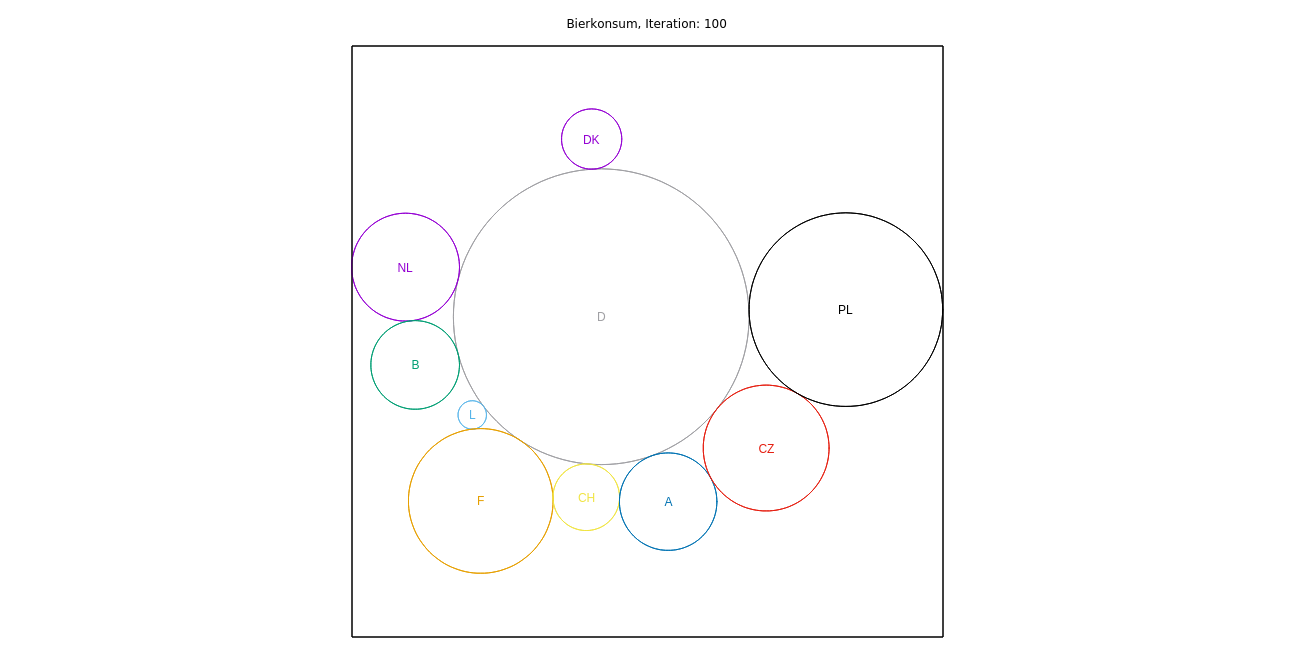
\includegraphics[width=\linewidth]{ihk_beispiel2.png}
\end{center}

Das obige Beispiel zeigt eine schematische Darstellung Mitteleuropas mit Deutschland und seinen Nachbarstaaten. Der Kennwert ist der Bierkonsum der einzelnen Staaten. Erkennbar ist, dass die Staaten nicht im Verh\"altnis
ihrer Fl\"ache sondern zum Kennwert dargestellt werden.
\subsection{Eingabedatei}
Zur Erstellung der Landkarte sollen \"uber eine Eingabedatei Daten eingelesen werden. Die Datei hat folgendes Format:
Die erste Zeile enth\"alt den Titel der Karte, z.B. "Fl\"ache der Staaten".
Zeilen, die mit "\#" beginnen, sind Kommentare und werden im weiteren Ablauf nicht betrachtet.
Nach dem ersten Kommentar folgen alle Staaten zeilenweise mit jeweils einem Staat pro Zeile. Dabei enth\"alt jede Zeile die folgenden Informationen:
\begin{itemize}
\item Autokennzeichen, z.B. "D" f\"ur Deutschland
\item Kennzahl
\item L\"angengrad
\item Breitengrad
\end{itemize}
Die Informationen sind jeweils durch Whitespace, Tab oder Leerzeichen, getrennt.
Auf die Liste der Staaten folgt ein Kommentar mit dem Hinweis, dass im Anschluss die Nachbarschaftsbeziehungen folgen. Jene folgen ebenfalls zeilenweise.
Die Nachbarschaftsbeziehungen werden bidirektional angegeben, d.h. ist ein Staat A ein Nachbar von Staat B, so ist automatisch auch B Nachbar von A.
Das Format der Nachbarschaftsbeziehungen sieht wie folgt aus:
\mybox{background}{$<$Kennz. Ausgangsland$>$: $<$Kennzeichen Nachbar 1$>$ $<$...$>$ $<$Kennzeichen Nachbar N$>$}
Die einzelnen Nachbarstaaten sind ebenfalls durch Whitespace (Leerzeichen oder Tab) getrennt. 
Grundsätzlich wird angenommen, dass das Format der Eingabedatei syntaktisch korrekt ist. Die Syntax wird daher nicht mehr auf Korrektheit \"uberpr\"uft.

\vspace{10mm}

\textbf{Beispiel:}\\
Die Eingabedatei vom vorherigen Beispiel k\"onnte wie folgt aussehen:\\
\vspace{5mm}
\mybox{background}{
Bierkonsum\\
\# Staat Fläche Längengrad Breitengrad\\
D 8692 10.0 51.3\\
NL 1156 5.3 52.2\\
B 781 4.8 50.7\\
L 80 6.1 49.8\\
F 2077 2.8 47.4\\
CH 440 8.2 46.9\\
A 945 14.2 47.6\\
CZ 1573 15.3 49.8\\
PL 3724 18.9 52.2\\
DK 360 9.6 56.0\\
\# Nachbarschaften\\
D: NL B L F CH A CZ PL DK\\
NL: B\\
L: F\\
F: CH\\
CH: A\\
A: CZ\\
CZ: PL
}
\subsection{Ausgabedatei}
Nach dem Einlesen der oben beschriebenen Daten und der Berechnung der Landkarte soll eine Ausgabe mit den berechneten Werten erstellt werden.
Diese soll dem folgenden Format gen\"ugen:
\mybox{background}{
reset
set xrange [$<$xmin$>$:$<$xmax$>$]
set yrange [$<$ymin$>$:$<$ymax$>$]\\
set size ratio 1.0\\
set title "$<$Name des Kennwertes$>$, Iteration: $<$nr$>$"\\
unset xtics\\
unset ytics\\
\$data $<<$ EOD\\
$<$Liste aus $<$xpos$>$ $<$ypos$>$ $<$radius$>$ $<$autokennzeichen$>$ $<$id$>$ $>$\\
EOD\\
plot \textbackslash\\
'\$data' using 1:2:3:5 with circles lc var notitle, \textbackslash\\
'\$data' using 1:2:4:5 with labels font \grqq{}arial,9\grqq{}  tc variable notitle\\
}
\\
\\
Die Intervalle \colorbox{lightgray}{[$<$xmin$>$:$<$xmax$>$]} und \colorbox{lightgray}{[$<$ymin$>$:$<$ymax$>$]} geben jeweils die kleinste und gr\"osste x- bzw. y-Koordinate der Landkarte an.
\colorbox{lightgray}{$<$Name des Kennwertes$>$} gibt den Namen des Kennwertes an, der in der Eingabedatei in der 1. Zeile angegeben wird.
Die Anzahl der Iterationen wird in \colorbox{lightgray}{$<$nr$>$} angegeben.
In der \colorbox{lightgray}{$<$Liste aus $<$xpos$>$ $<$ypos$>$ $<$radius$>$ $<$autokennzeichen$>$ $<$id$>$ $>$} werden alle Staaten nacheinander aufgelistet. Die Werte
\colorbox{lightgray}{$<$xpos$>$ und $<$ypos$>$} sind die Koordinaten des jeweiligen Kreismittelpunktes, der \colorbox{lightgray}{$<$radius$>$} ist der ermittelte Radius des Kreises.
Das \colorbox{lightgray}{$<$autokennzeichen$>$} gibt das Kennzeichen des Staats an und die \colorbox{lightgray}{$<$id$>$} ist eine fortlaufende Nummerierung beginnend bei 0, die f\"ur die 
Farbgebung in Gnuplot erforderlich ist.\\
\vspace{40mm}\\
\textbf{Beispiel:}\\
\vbox{
Die Ausgabe f\"ur das Beispiel \glqq{}Bierkonsum\grqq{} k\"onnte wie folgt aussehen:\\
\mybox{background}{
reset\\
set xrange[122.2902588107926:332.4746754411094]\\
set yrange[990.7016847962033:1200.88610142652]\\
set size ratio 1.0\\
set title "Bierkonsum, Iteration: 100"\\
unset xtics\\
unset ytics\\
\$data << EOD\\
211.053730834 1104.45871827 52.5999004819 D 0\\
141.472704651 1122.09603019 19.1824458406 NL 1\\
144.871946688 1087.31207915 15.7670549282 B 2\\
165.183777819 1069.53934032 5.04626504404 L 3\\
168.191312507 1038.92448868 25.7124412222 F 4\\
205.719560567 1040.2435555 11.8345405454 CH 5\\
234.860729713 1038.69277989 17.3436686558 A 6\\
269.709149473 1057.75886679 22.3763591982 CZ 7\\
298.045240126 1106.99471738 34.4294353156 PL 8\\
207.661916065 1167.67099407 10.7047446969 DK 9\\
EOD\\
plot \textbackslash \\
'\$data' using 1:2:3:5 with circles lc var notitle, \textbackslash \\
'\$data' using 1:2:4:5 with labels font \grqq{}arial,9\grqq{} tc variable notitle\\
}
}
\subsection{Spezial- und Sonderf\"alle bei der Eingabe}
Syntaxfehler in der Eingabedatei sind laut Aufgabenstellung ausgeschlossen. Daher benutze ich als Format f\"ur meine Eingabedatei restriktiv das unter Punkt 1.1 angegebene Format,
inklusive der Kommentarzeilen.\\ Den Inhalt der Kommentarzeilen ignoriere ich, allerdings benutze ich sie zur Orientierung beim Einlesen der Zeilen. Vor dem ersten Kommentarzeichen, das ein \# ist, befindet sich
der Titel, auf den ersten Kommentar folgen die Staaten und nach dem zweiten Kommentar kommen die Nachbarschaftsbeziehungen.\\ \\ \textbf{Vorschriften}:\\
\vspace{3mm}
\begin{itemize}
\item Doppelt vorkommende Autokennzeichen sind nicht erlaubt, da diese eindeutig sein m\"ussen, um einen Staat eindeutig identifizieren zu k\"onnen.\\
\item Zwei mal der selbe Mittelpunkt f\"ur zwei verschiedene Staaten ist nicht erlaubt. \\
\item Der Kennwert muss mindestens 1 sein.
\item Kennwerte sollten nicht zu gross gew\"ahlt werden, weil das Koordinatensystem durch den gew\"ahlten Datentyp
double beschr\"ankt ist und es ansonsten in Ausnahmef\"allen durch die berechneten Kr\"afte zu einer \"Uberschreitung des erlaubten Wertebereichs kommen k\"onnte. In diesem Fall w\"are es erforderlich die Kennzahl anzupassen, bpsw. durch eine \"Anderung der Gr\"ossenordnung.
\item Die L\"angen- und Breitengrade m\"ussen im Wertebereich des \textit{World Geodetic System 1984 (WGS84)} liegen. Das bedeutet, dass die Breitengrade im Intervall [-90;+90] liegen m\"ussen und L\"angengrade im Intervall [-180;+180].
Andere Werte werden nicht akzeptiert.
\item Alle Staaten m\"ussen zusammenh\"angen. Ansonsten ist die Berechnung nicht durchf\"urbar.
\end{itemize}
\section{Objektorientierter Entwurf}
\subsection{Klassendiagramm}
\begin{center}
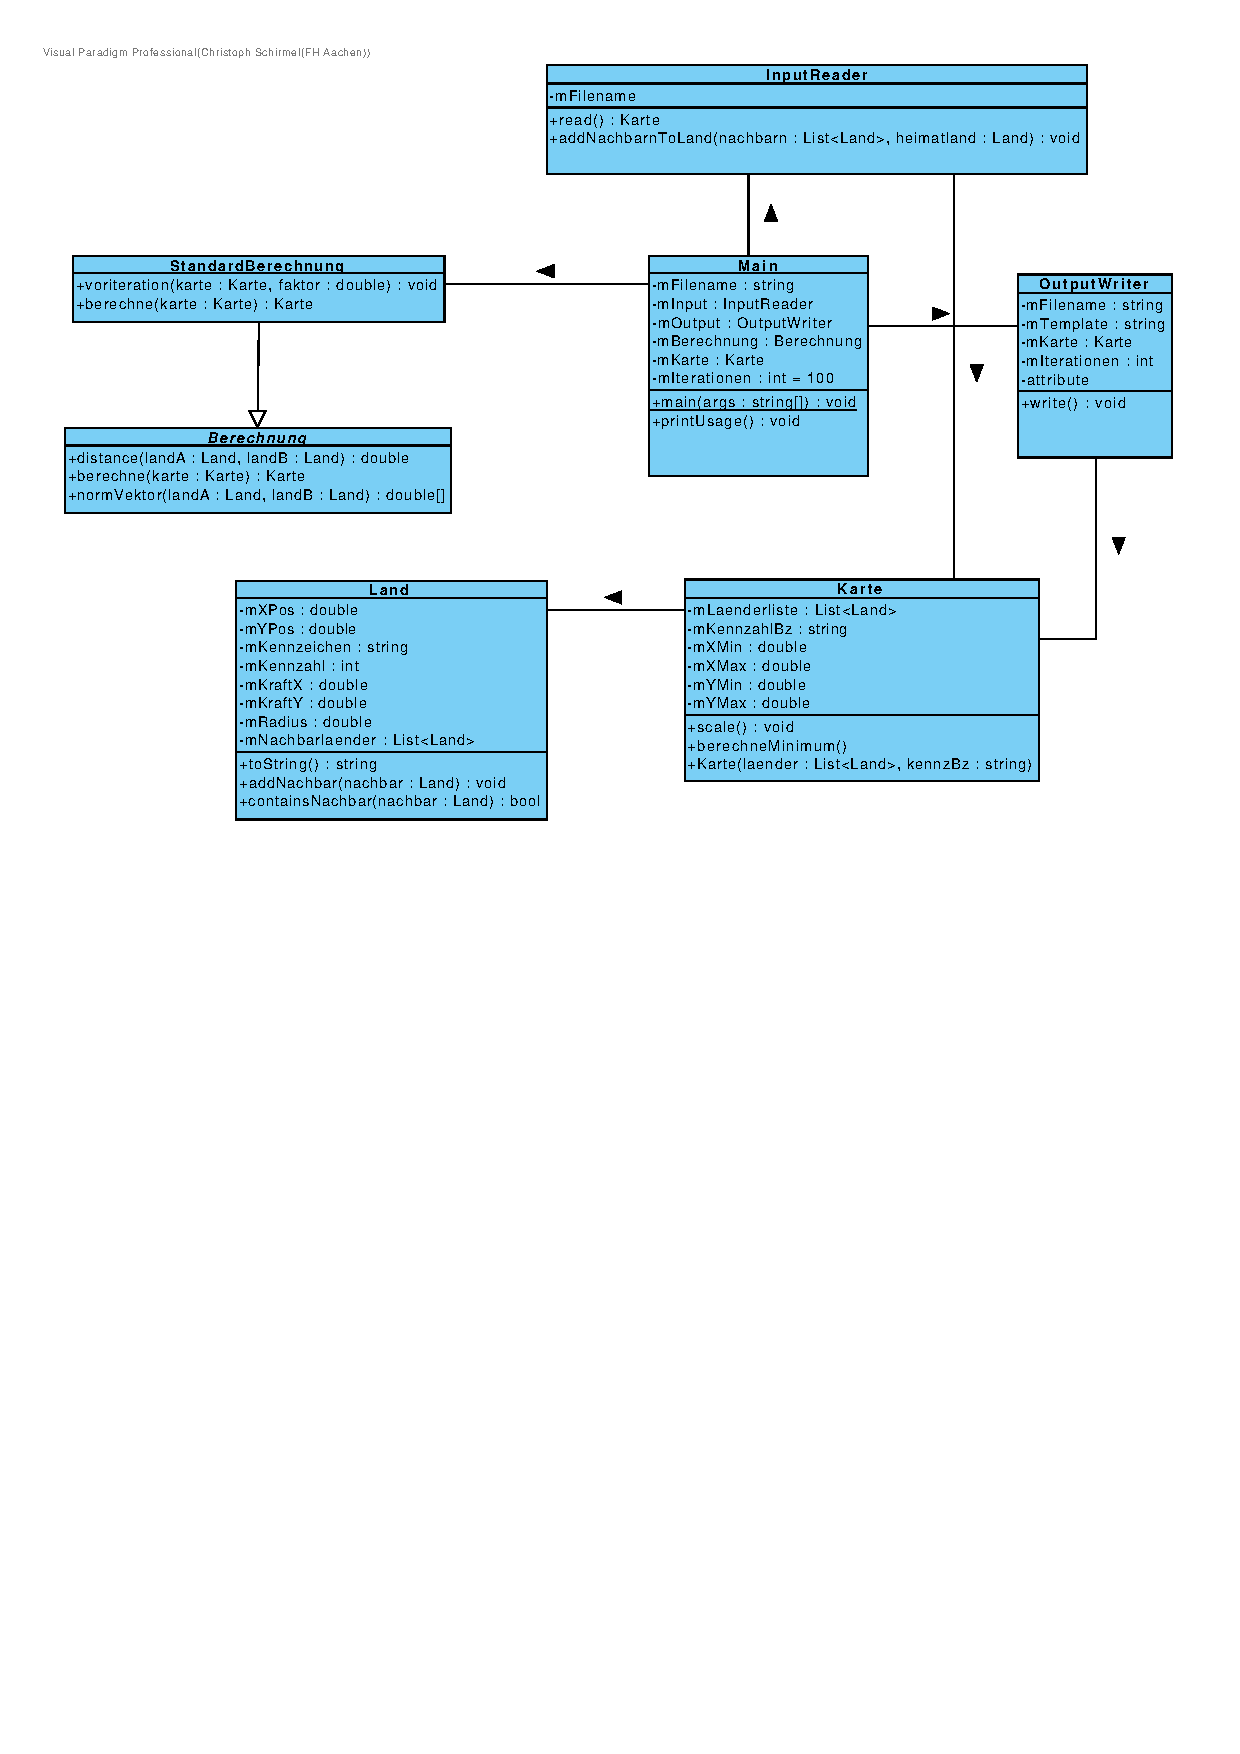
\includegraphics[width=\linewidth]{klassendiagramm_gropro.pdf}
\end{center}
\subsection{Beschreibung}
Die Hauptklasse des Programms ist die Klasse \colorbox{lightgray}{Main}, die den Einstiegspunkt des Programms markiert und alle anderen Vorg\"ange steuert.
Hierf\"ur hat sie \"uber ihre Attribute Zugriff auf die Funktionen f\"ur Ein- und Ausgabe, die Berechnung und die zurzeit eingelesenen Daten. Auch die Anzahl der 
Iterationen, die berechnet werden sollen, werden in der Klasse Main gespeichert.
Das zeilenweise Einlesen der Eingabedatei ist in der Klasse \colorbox{lightgray}{InputReader} in der Methode \colorbox{lightgray}{read} implementiert, die ein Objekt der
Container-Klasse \colorbox{lightgray}{Karte} zur\"uckgibt. In einem Objekt von Karte sind die Minima und Maxima des aktuellen Wertebereichs, sowie alle Informationen \"uber alle eingelesenen L\"ander und die Bezeichnung der Kennzahl gespeichert.
S\"amtliche Informationen \"uber ein \colorbox{lightgray}{Land} werden in der gleichnamigen Klasse gespeichert. Diese sind jeweils das Autokennzeichen des Landes, die Nachbarlaender, welche in einer Liste abgelegt werden,
der Radius des Kreises, der sich aus der ebenfalls gespeicherten Kennzahl ergibt und die Summe aller wirkenden Anziehungs- und Abstossungskr\"afte, die jeweils w\"ahrend einer Iteration gespeichert werden.
Der Kern des Programms, befindet sich in der Klasse \colorbox{lightgray}{Berechnung} bzw. \colorbox{lightgray}{Standardberechnung}. Hier wird in der Methode \colorbox{lightgray}{berechne}, die den Hauptalgorithmus implementiert die \glqq eigentliche\grqq{}
Berechnung der neuen Kreismittelpunkte durchgef\"uhrt. Der Hauptalgorithmus greift zus\"atzlich auf die Hilfsmethoden \colorbox{lightgray}{voriteration}, \colorbox{lightgray}{normVektor} und \colorbox{lightgray}{distance} zu.

\subsection{Ablauf Eingabe}
Das Einlesen der Eingabedatei l\"auft wie folgt ab:\\
Zuerst wir die Eingabedatei zum Lesen ge\"offnet. Zeilenweise wird nun der Inhalt der Datei eingelesen. Das Format der Datei muss dabei dem vorgegebenen Format entsprechen (vgl. Punkt 1.1 Eingabedatei).
\"Uber eine Z\"ahlvariable wird bestimmt, welche Informationen als n\"achstes eingelesen werden. Zu Beginn hat diese Z\"ahlvariable den Wert 0.
Wenn die Variable 0 ist, muss die n\"achste Zeile die erste Zeile der Datei sein. Diese enth\"alt die Bezeichnung der Kenngr\"osse und wird in eine tempor\"are Variable gespeichert und anschliessend erh\"oht sich der Z\"ahler um 1.
Bei jedem Kommentar wird der Z\"aehler ebenfalls erh\"oht. Da sich zwischen der ersten Zeile und dem Einlesen der L\"ander ein Kommentar befindet, hat der Z\"ahler beim Einlesen der L\"ander den Wert 2.
Wenn also der Z\"ahler gleich 2 ist, werden die L\"ander nacheinander eingelesen. Die Zeile wird gesplittet, sodass in einer Liste alle Informationen (Kennzeichen, Kennzahl, L\"angen- und Breitengrad) einzeln vorliegen.
Hier wird nun \"uberpr\"uft, ob die angegebenen Werte korrekt sind, also ob die Kennzahl gr\"osser als 1 ist, L\"angen- und Breitengrade im entsprechenden Intervall liegen usw. 
Wenn nicht, wird ein Fehler ausgel\"ost, der das Programm mit einer Meldung an den Benutzer beendet. Sind alle Werte korrekt, wird ein neues Objekt der Klasse \colorbox{lightgray}{Land} erzeugt, das dann in
einer L\"anderliste zwischengespeichert wird. Dies l\"auft f\"ur alle L\"ander gleich ab.
Nach den L\"andern folgt ein Kommentar, der den Z\"ahler auf 3 erh\"oht. Das bedeutet, dass als n\"achstes die L\"anderbeziehungen eingelesen werden.
Hier wird f\"ur jede Zeile am Doppelpunkt aufgeteilt zwischen Ausgangsland und dessen Nachbarn. Im Anschluss werden dem Ausgangsland seine Nachbarn zugeordnet und
gleichzeitig jedem Nachbarn das Ausgangsland als Nachbar zugeordnet.\\
Aus der L\"anderliste und der Bezeichnung der Kenngr\"osse wird ein Objekt der Klasse Karte erzeugt. Dieses wird zur\"uckgegeben.

\begin{center}
\vbox{
	Methode read() aus Klasse InputReader\\
	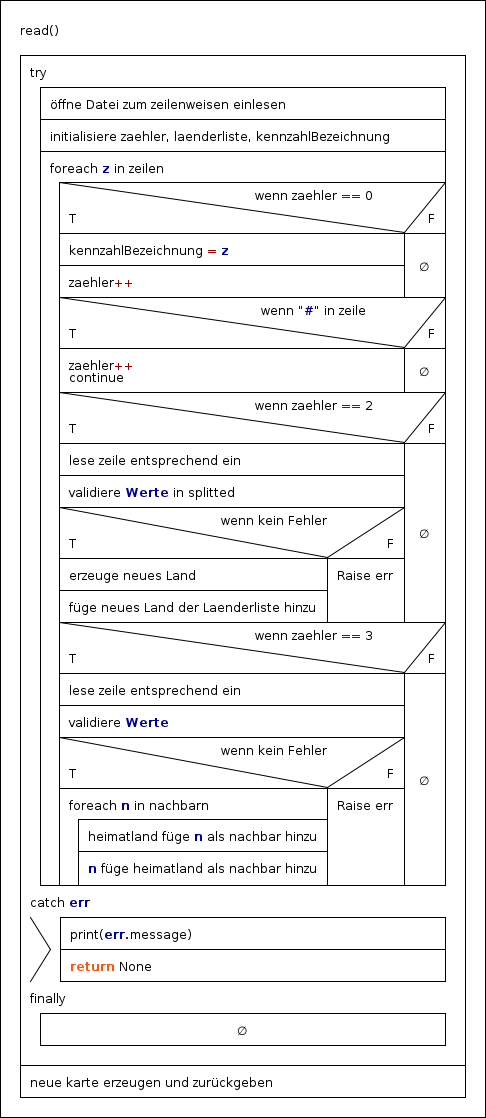
\includegraphics[scale=0.5]{read.png}
}
\end{center}
\subsection{Ablauf Ausgabe}
F\"ur die Ausgabe wird ein Template eingelesen, das der allgemeinen Form der Aufgabenstellung (Siehe Punkt 1.2 Ausgabedatei) entspricht eingelesen. Alle Tags werden 
durch die entsprechenden Werte ersetzt, wobei f\"ur den Tag $<$Liste aus ...$>$ ein String erstellt wird, der alle L\"ander enth\"alt. Zuletzt wird die Datei unter dem neuen Namen
abgespeichert. Dieser entspricht dem Eingabenamen und der Endung ".gpl" oder einem per Parameter frei gew\"ahlten Namen.

\begin{center}
	\vbox{
		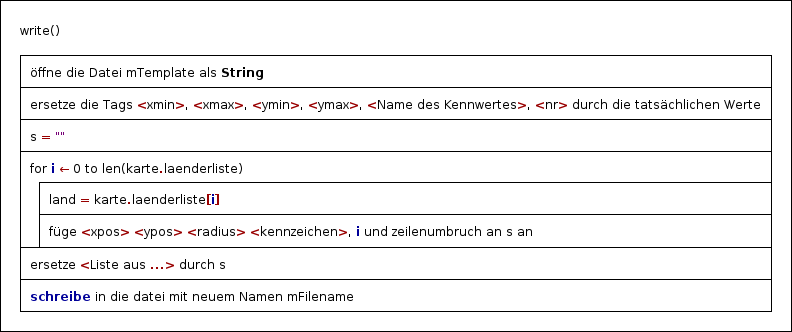
\includegraphics[width=\linewidth]{write.png}
	}	
\end{center}


\subsection{Ablauf Hauptalgorithmus}

\subsubsection{Voriteration}

Vor der ersten Iteration wird eine Voriteration durchgef\"uhrt, um das Endergebnis zu verbessern. Bei der Voriteration soll der Abstand zwischen den L\"andern
vergr\"ossert werden, ohne das Verh\"altnis der L\"ander zu beeinflussen.
Hierf\"ur habe ich mir zwei Ans\"atze \"uberlegt:\\
Der erste Ansatz vergr\"ossert die Abst\"ande, indem alle Mittelpunkte um einen Faktor x skaliert werden. Der Faktor ist grunds\"atzlich erstmal eine positive reelle Zahl
gr\"osser bzw. gleich 1 (falls keine Voriteration gewollt ist). Die hierdurch erzielten Ergebnisse waren insbesondere beim dritten Beispiel der IHK besser, f\"uhrten allerdings
je nach gew\"ahltem Faktor auch zu zu grossen Zahlen und dadurch zu einem unbrauchbaren Ergebnis.
Daher habe ich mir einen anderen Ansatz \"uberlegt, der auch besser funktioniert, n\"amlich die Verkleinerung der Radien. Hierf\"ur habe ich alle Radien zuerst mit einem
Faktor x$>$1 (default = 2) multipliziert und anschliessend durch den kleinsten Radius geteilt.
\vspace{3mm}
\begin{center}
	\vbox{
		Voriteration 1: Skalieren der Kreismittelpunkte\\
		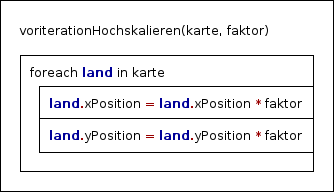
\includegraphics[width=0.6\linewidth]{voriterationHochskalieren.png}
	}
	\vspace{5mm}
	\vbox{
		Voriteration 2: Skalieren der Radien\\
		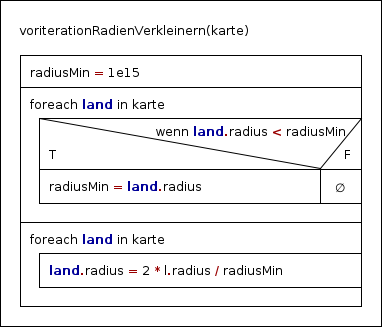
\includegraphics[width=0.6\linewidth]{voriterationRadienVerkleinern.png}
	}
\end{center}


\subsubsection{Hauptalgorithmus}
Der Hauptalgorithmus zur Bestimmung der Abstossungs- und Anziehungskr\"afte ist wie in der Aufgabenstellung angegeben ein Iterationsverfahren.
Es bekommt die aktuelle geographische Lage als Karte \"ubergeben. Dabei handelt es sich entweder um die Ausgangslage nach der Voriteration oder aber um das Ergebnis
der letzten Iteration. Der Hauptalgorithmus wird so oft ausgef\"uhrt wie Iterationen N (default=100) angegeben werden. Der Hauptalgorithmus berechnet f\"ur jeden Staat
dessen Anziehungs- und Abstossungskr\"afte zu allen Nachbarstaaten bzw. zu Staaten, die von ihm geschnitten werden. Dabei gilt f\"ur die Kraft F von einem Staat A zu einem Staat B
folgende Formel:\\
\begin{center}
\LARGE{$ F = \frac{|r_{A}+r_{B}+|\vec{d_{BA}}||}{g * |\vec{d_{AB}|}} * \vec{d_{BA}}$}
\end{center}
\vspace{5mm}
Bei g handelt es sich um eine Konstante, die die Kr\"afte anteilig auf die beiden Staaten verteilt, sodass nicht beide die volle Kraft aufaddiert bekommen und nicht einer allein die ganze Kraft.
In der Aufgabenstellung wurde vorgeschlagen die Kraft h\"alftig zu verteilen. Ich habe im Praxiseinsatz festgestellt, dass meine Implementierung besser funktioniert, wenn g$<$0.5 ist und habe einen
Standardwert von 0.3 festgelegt. Die berechneten Kr\"afte werden auf den Kraftvektor des jeweiligen Landes addiert, weil f\"ur die Gesamtkraft, die auf ein Land A wirkt, gilt:\\
\begin{center}
\LARGE{$ F_{A} = \sum_{i=1}^{n} F_{i} $}
\end{center}
\vspace{5mm}
wobei $ F_{i}$ alle auf das Land A wirkende Kr\"afte sind.\\

Nach dem Berechnen werden alle Kr\"afte auf die Mittelpunkte der Kreise angewandt und so die \glqq{}neuen\grqq{} Mittelpunkte berechnet. Der gesamte Ablauf
wird im folgenden in einem Nassi-Shneiderman-Diagramm dargestellt:

\begin{center}
	\vbox{
		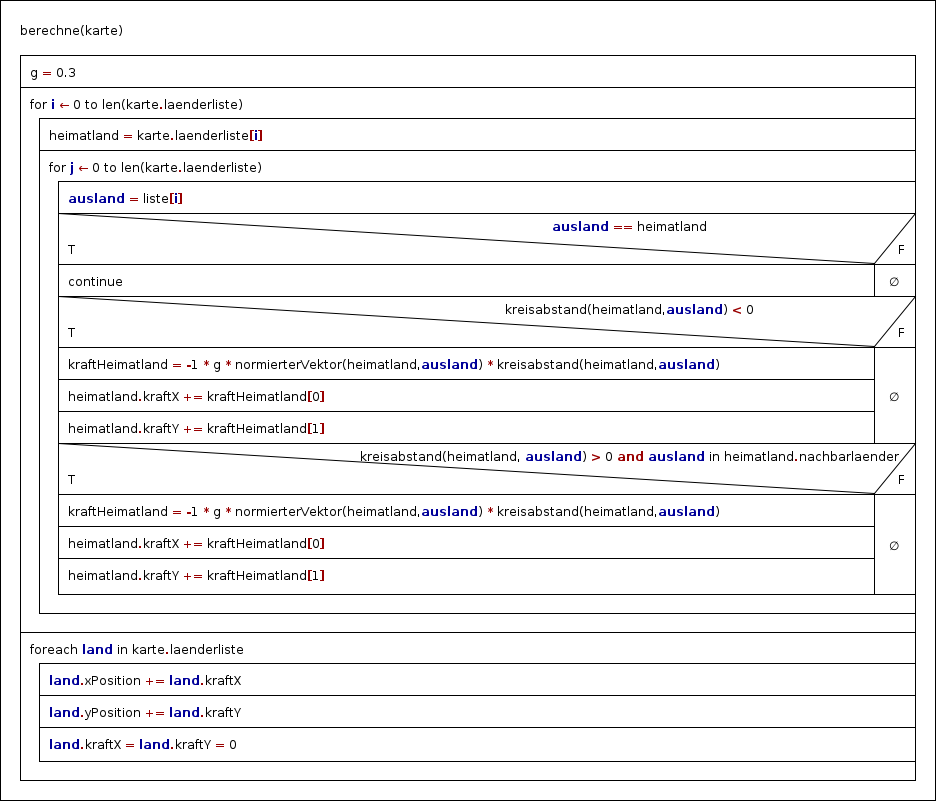
\includegraphics[width=\linewidth]{berechne.png}
	}
\end{center}




\subsection{Sequenzdiagramm}

\vbox{
	\begin{center}
		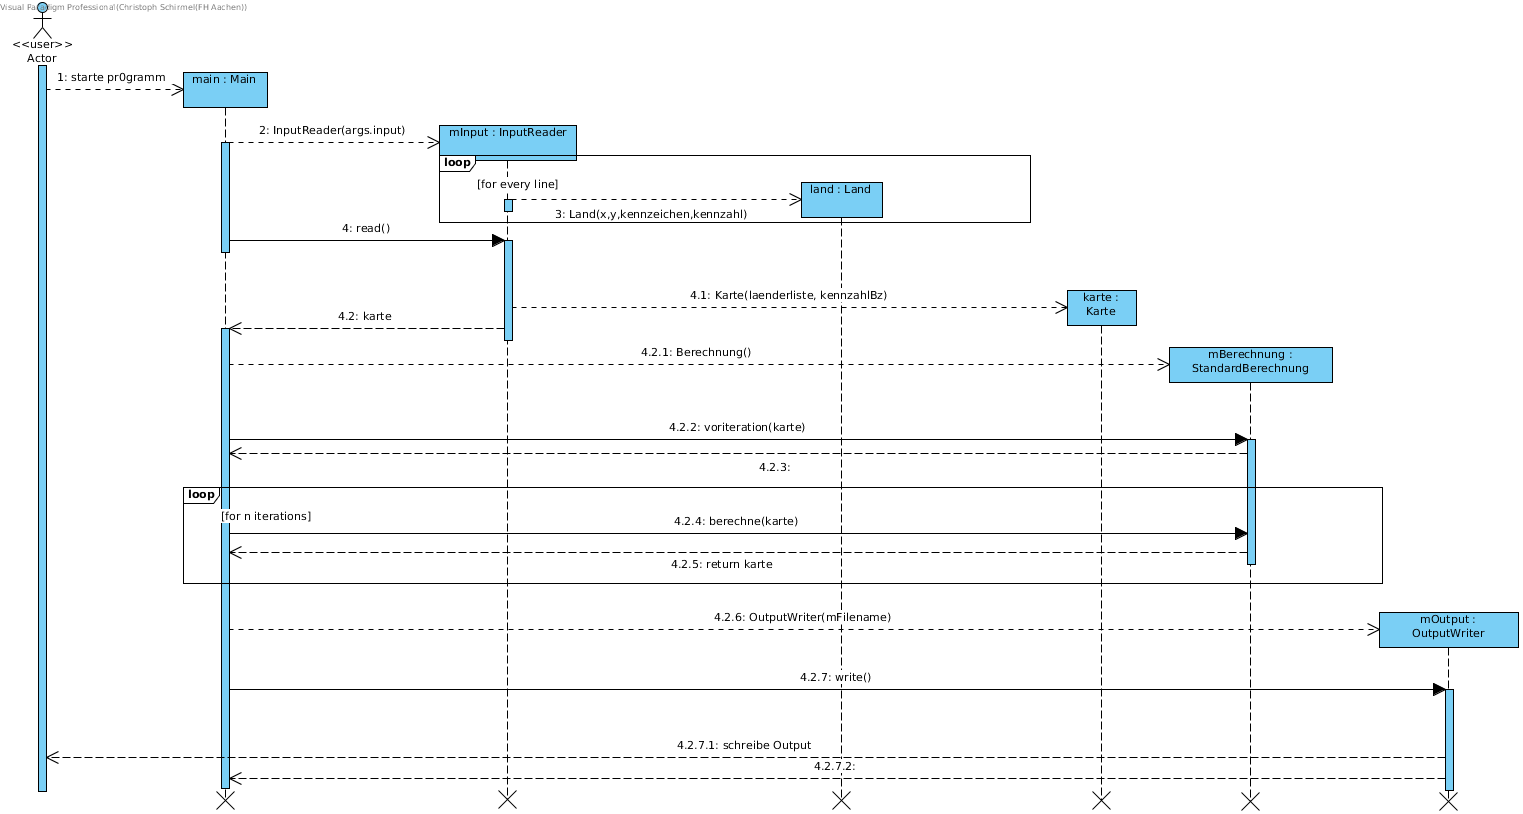
\includegraphics[width=\linewidth]{Sequenzdiagramm.png}
	\end{center}
}

\section{\"Anderungen zum Montagsteil}
\subsection{\"Anderungen in der Klassenstruktur}

Die Klassenstruktur wurde auf die Programmiersprache angepasst, ist aber grunds\"atzlich erhalten geblieben. Aus dem Interface Berechnung habe ich eine abstrakte Klasse gemacht, um sinnvolle Methoden abstrahieren zu k\"onnen. Da ich in Python gearbeitet habe, waren Getter und Setter nicht mehr erforderlich, da alle Variablen, die ausserhalb von Funktionen definiert sind global sind.
Im Klassendiagramm wurden in der Klasse \colorbox{lightgray}{Land} die beiden Membervariablen \colorbox{lightgray}{radius} und \colorbox{lightgray}{nachbarlaender} eingef\"ugt.
Ausserdem habe ich die folgenden Methoden erg\"anzt:

\textbf{Klasse InputReader:}\\
\begin{itemize}
	\item \colorbox{lightgray}{zusammenhaengend(laenderliste)} - Wrapper um Rekusionsaufruf
	\item \colorbox{lightgray}{zusammenhaengendRek(startland, besucht)} - rekursive Methode, die ermittelt, ob alle L\"ander zusammenh\"angen
	\item \colorbox{lightgray}{addNachbarnToLand} - f\"ugt einem Land einen Nachbar hinzu.\\
\end{itemize}
\textbf{Klasse Karte:}\\
\begin{itemize}
	\item \colorbox{lightgray}{scale()} - Erf\"ullt die Bedingung ymax-ymin = xmax-xmin
	\item \colorbox{lightgray}{berechneMinimum()} - Berechnet die Minima xmin, ymin und Maxima xmax, ymax
\end{itemize}
\textbf{Klasse Land:}\\
\begin{itemize}
	\item \colorbox{lightgray}{\_\_str\_\_()} - Stringdarstellung eines Landes
	\item \colorbox{lightgray}{\_\_repr\_\_()} - Stringdarstellung eines Landes (f\"ur debugging)
	\item \colorbox{lightgray}{addNachbar(nachbar)} - F\"ugt einen Nachbar hinzu
	\item \colorbox{lightgray}{containsNachbar(nachbar)} - Gibt true zur\"uck wenn nachbar Nachbar ist
\end{itemize}
\textbf{Klasse \textit{Berechnung:}}\\
\begin{itemize}
	\item \colorbox{lightgray}{distance(landA, landB)} - Berechnet den Kreisabstand zwischen zwei L\"andern
	\item \colorbox{lightgray}{normVektor(landA, landB)} - Gibt den normierten Verbindungsvektor AB zur\"uck
\end{itemize}
\textbf{Klasse Standardberechnung:}
\begin{itemize}
	\item \colorbox{lightgray}{mittelwertRadien(karte)} - Gibt den Mittelwert der Radien zur\"uck
	\item \colorbox{lightgray}{voriteration} - f\"uhrt eine Voriteration durch
\end{itemize}



\subsection{\"Anderungen beim Algorithmus}
An meinem Hauptalgorithmus habe ich im Vergleich zu Montag so ver\"andert, dass die \"Uberpr\"ufung weggefallen ist, ob eine Kraft bereits h\"alftig auf ein Land angewandt wurde oder nicht.
Dies habe ich dadurch ersetzt, dass nun \"uber alle L\"ander iteriert wird und von vornherein nur die anteilige Kraft angewandt wird. Die beiden m\"oglichen Voriterationen wurden nach Montag ebenfalls eingef\"ugt.
Die Kraft wird anteilig mit einem Faktor von 0.3 auf beide Mittelpunkte angewandt. Dies verbesserte das Ergebnis im Vergleich zu 0.5.

\section{Zusammenfassung und Ausblick}
Das Programm funktioniert wie in der Aufgabenstellung vorgegeben: Es liest die syntaktisch korrekte Datei ein, pr\"uft auf semantische Fehler wie z.B. ein doppeltes Land, berechnet die geforderte Anzahl
Iterationen und schreibt das Ergebnis in eine Ausgabedatei. Intern werden durch einen objektorientierten Ansatz Ein-/Ausgabe und Funktionalit\"at sauber voneinander getrennt und \"uber eine Abstrahierung
der Klasse Berechnung ist es leicht m\"oglich weitere Klassen zur Berechnung abzuleiten.

Ausblick-Ideen: GUI, Parallelisierung, weitere Features


\section{Benutzeranleitung}
\subsection{Ordnerstruktur}
Die .zip Datei beinhaltet die Sourcen mit der Main.py als Hauptklasse zum Ausf\"uhren, ein Testskript und diese Dokumentation. Außerdem sind die Ordner \glqq docu\grqq{} und \glqq tests\grqq{} enthalten.
Im \glqq docu\grqq{}-Ordner befindet sich ein PDF-Dokument mit der API, die mit epydoc generiert wurde. In dem tests Ordner befinden sich die Testf\"alle.\\
\vspace{2mm}
Ordnerstruktur:\\
\mybox{background}{
	- LandkartenDoku.pdf (dieses Dokument)\\
	- readme.md (Eine Benutzeranleitung im Markdown Format)\\
	- run\_all\_tests.py (Das Skript zum Ausf\"uhren der Tests)\\
	- Main.py (Die Hauptklasse)\\
	- Land.py\\
	- Karte.py\\
	- Berechnung.py\\
	- InputReader.py\\
	- OutputWrite.py\\
	- \textbackslash doc\\
	- \textbackslash tests
}
\subsection{Voraussetzungen}
Zum Ausf\"uhren wird \href{https://www.python.org/}{Python} ben\"otigt. Das Programm wurde sowohl mit Version 2.7 als auch 3.7.3 getestet. Python ist frei benutzbar und l\"auft unter der
\textit{Python-Software-Foundation-Lizenz}, die kompatibel mit der GNU General Public License ist.\\
Des weiteren muss zum Ausf\"uhren die unter der BSD-Lizenz ver\"offentlichte Bibliothek \href{https://www.numpy.org/}{NumPy} installiert sein.
Falls diese nicht installiert ist, kann sie \"uber die Kommandozeile einfach installiert werden:\\
\colorbox{lightgray}{pip install numpy}\\

Zum Erstellen der Grafiken kann optional das Programm Gnuplot installiert werden.

\subsection{Laufzeitumgebung}
Die Software wurde auf Windows 10 Education und Ubuntu Bionic Beaver 18.04 LTS auf 64-bit entwickelt. Als Entwicklungsumgebung wurde \textit{Visual Studio Code Version 1.33}
mit der mitgelieferten Python Extension benutzt. 

\subsection{Installation}

%if python
Eine Installation ist nicht notwendig, weil die benutzte Sprache Python eine Interpretersprache ist. Die Dateien werden zur Laufzeit vom Interpreter in ausf\"uhrbaren Code \"ubersetzt.


\subsection{Ausführen des Programms}
\subsubsection{Direkt}
F\"ur den direkten Aufruf kann folgender Befehl verwendet werden:\\
\colorbox{lightgray}{python Main.py -i INPUT [-n ITERATIONEN $|$ -s Skalierungsfaktor $|$ -o OUTPUT]}

\subsubsection{Mit dem Skript}
Mit dem Skript \colorbox{lightgray}{run\_all\_tests.py} k\"onnen alle in einem Ordner liegenden Tests ausgef\"uhrt werden. Als erstes Argument wird der Pfad zur Datei \colorbox{lightgray}{Main.py} erwartet. Das zweite Argument
ist optional der Pfad zu einem Ordner mit Inputdateien. Falls der angegebene Pfad nicht erreicht werden kann, wird stattdessen der lokale Ordner \colorbox{lightgray}{tests}
verwendet. Das Skript f\"uhrt die Berechnung mit den Standardparametern aus, die i.d.R. ein passables Testergebnis liefern.\\
Windows: \colorbox{lightgray}{python .$\backslash$ run\_all\_tests.py .$\backslash$Main.py}\\
Linux: \colorbox{lightgray}{python ./run\_all\_tests.py ./Main.py}\\
\subsection{Restriktionen beim Dateinamen}
Die Datei muss dem benutzten Betriebssystem entsprechend einen g\"ultigen Dateinamen besitzen.
Sie kann sowohl \"uber den relativen Pfad ausgehend vom Ordner des Aufrufs als auch \"uber den absoluten Pfad angegeben werden.
Die Pfade m\"ussen auch dem Format des benutzten Betriebssystem entsprechen.
Beispiele f\"ur Dateipfade:
\vspace{3mm}
Absoluter Pfad:\\
\colorbox{lightgray}{Windows: python \glqq C:$\backslash$Users$\backslash$User$\backslash$Documents$\backslash$gropro$\backslash$Main.py\grqq{}}\\
\colorbox{lightgray}{Linux: python /home/user/documents/gropro/Main.py}\\
Relativer Pfad:\\
\colorbox{lightgray}{Windows: python .$\backslash$Main.py}\\
\colorbox{lightgray}{Linux: python ./Main.py}


\subsection{Anmerkung}

\section{Tests}

\subsection{IHK Tests}

\subsubsection{IHK Example 01 etc.}

\subsection{Funktionierende Tests}

\subsubsection{F01 bliblablub etc.}

\subsection{Syntax-Fehler Tests}

\subsubsection{S01 lirumlarum}

\subsection{Logik Fehler Tests}

\subsubsection{L01 loremipsum}

\subsection{Optional: Code Coverage Tests, Performance o.ae}

\section{Source-Code}
\begin{center}

\vbox{
Land.py\\
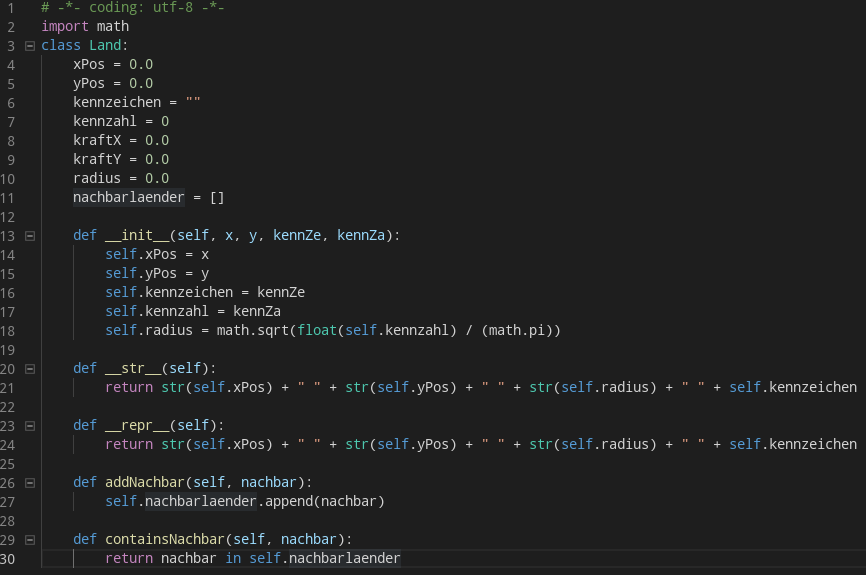
\includegraphics[width=\linewidth]{klasse_land_source.png}
}
\vbox{
OutputWrite.py\\
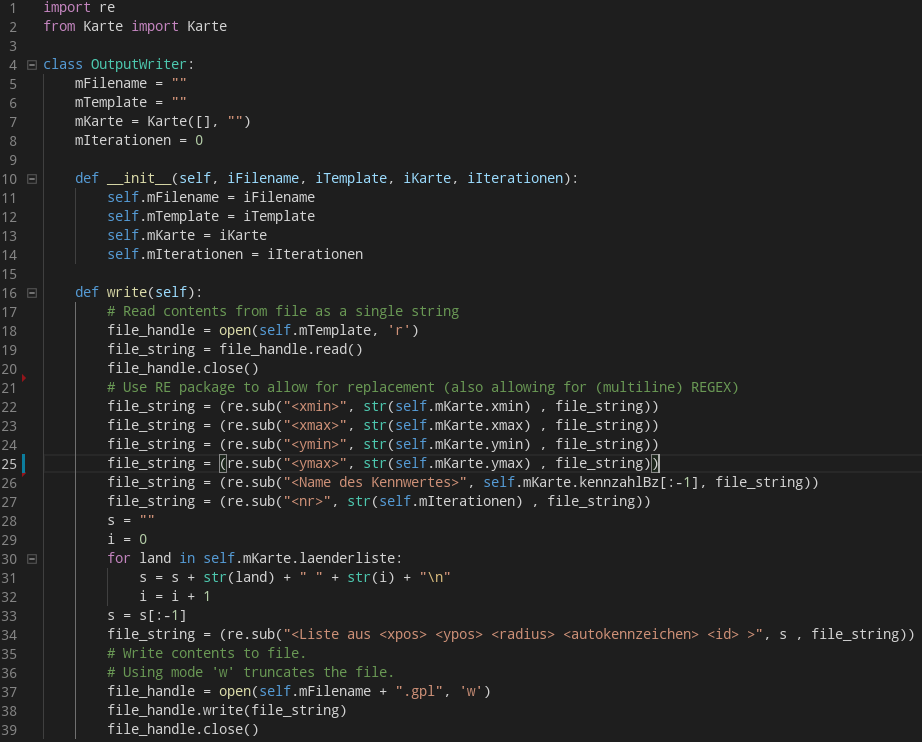
\includegraphics[width=\linewidth]{klasse_outputwrite_source.png}
}
\vbox{
Karte.py\\
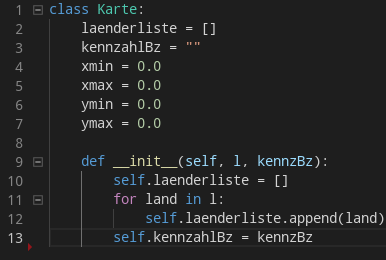
\includegraphics[scale=0.8, width=0.7\linewidth]{klasse_karte_source.png}
}

\end{center}

\lstset{
	basicstyle=\scriptsize\ttfamily,
	language=c++,
	frame=tb,
	tabsize=4,
	showstringspaces=false,
	numbers=left,
	commentstyle=\color{commentgreen},
	keywordstyle=\color{blue},
	stringstyle=\color{orange},
	breaklines=true
}

%\lstinputlisting[language=c++]{../main.cpp}
\end{document}
